\section{\LaTeX?}
\begin{frame}{Geschichte}
    \begin{columns}
        \column{0.5\textwidth}


    \begin{itemize}
        \item Donald Knuth hat 1977-1986 \TeX gemacht, da er die typografische Qualit\"at seiner B\"ucher nicht gut fand. (The Art of Computer Programming)

    \end{itemize}
        
        \hfill
        \column{0.5\textwidth}
        \begin{figure}[htpb]
            \centering
            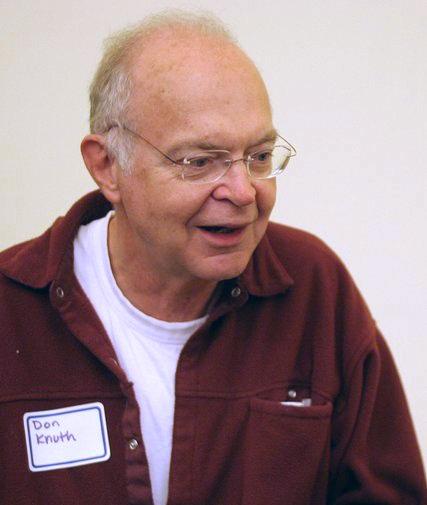
\includegraphics[width=0.7\textwidth]{./figs/tex-knuth.jpg}
        \end{figure}
    \end{columns}
\end{frame}

\begin{frame}{Was ist \LaTeX?}
    \begin{itemize}
        \item Textsatzystem.
        \item Erm\"oglicht Erstellen von Dokumenten.
        \item Beliebt im Akademischen Bereich/Wissenschaft.
        \item Erstellt hochwertige PDF Ausgabe.
    \end{itemize}
    
\end{frame}



\begin{frame}{Warum \LaTeX?}
    \begin{itemize}
        \item Ist sehr intuitiv.
        \item Sehr extensiv mit packages.
        \item K\"ummert sich um viel von alleine
        \item Man muss sich nicht mit Typografie und Vergleichbarem vertraut machen\footnote{Es funktioniert einfach und sieht gut aus.}.
        \item Macht spa\ss
    \end{itemize}
\end{frame}



\begin{frame}{Warum nicht Word? (oder andere WYSIWYG\footnote{WYSIWYG = What you see is what you get} software)}
    \begin{itemize}
        \item Word macht es schwerer \"Anderungen an gro\ss{}en Dokumenten vorzunehmen.
        \item Bibliografien werden nicht automatisch gemacht, auch Zitierstil nachtr\"aglich \"anderbar.
        \item Seitenzahlen, Referenzen, etc. werden nicht automatisch erzeugt.
        \item \textit{kann man nicht in Vim benutzen.}
    \end{itemize}
    
\end{frame}




\begin{frame}{Nutzzwecke}

    \begin{itemize}
        \item Ausarbeitungen/Laborberichte
        \item Pr\"asentationen
        \item Dokumente
        \item Lebenslauf
        \item B\"ucher
    \end{itemize}
\end{frame}





